
\begin{document}

%----------------------------------------------------------------------------------------
%	TITLE PAGE
%----------------------------------------------------------------------------------------

\title[Medical AI]{\huge{Medical AI}  \\
\medskip
\small{京东健康工作的回顾}
} % The short title appears at the bottom of every slide, the full title is only on the title page

% \author[文豪]{文豪} % Your name

% \institute[北京航空航天大学] % Your institution as it will appear on the bottom of every slide, may be shorthand to save space
% {
% 数学科学学院 \\ % Your institution for the title page
% \medskip
% \textit{wenh06@gmail.com} % Your email address
% 北京航空航天大学 \\
% 数学科学学院 \qquad 北京航空航天大学
% }

% \logo{\includegraphics[height=1.5cm]{logo}}
% \logoii{\includegraphics[height=1cm]{logo2}}

% \date{\footnotesize 2021年4月13日} % Date, can be changed to a custom date

\setlength{\belowdisplayskip}{5pt} \setlength{\belowdisplayshortskip}{5pt}
\setlength{\abovedisplayskip}{5pt} \setlength{\abovedisplayshortskip}{5pt}

%------------------------------------------------

\begin{frame}
\titlepage % Print the title page as the first slide
\end{frame}

%------------------------------------------------

\begin{frame}
% \frametitle{Overview} % Table of contents slide, comment this block out to remove it
\tableofcontents % Throughout your presentation, if you choose to use \section{} and \subsection{} commands, these will automatically be printed on this slide as an overview of your presentation
\end{frame}

%------------------------------------------------

%------------------------------------------------
%	PRESENTATION SLIDES
%------------------------------------------------


% PPT version (read only share link): https://www.kdocs.cn/l/cigmbsd3uAI4

%------------------------------------------------

\section{Physiological Signal Processing}

%------------------------------------------------
% Page 1

\begin{frame}
\frametitle{深度学习应用于生理信号处理}

\uncover<2->{生理信号主要包括:心电ECG,脉搏波PPG}
\vspace{1em}

\uncover<3->{我们在京东健康创建了一套非常完整的ECG分析系统,\\}
\uncover<4->{传统信号处理、机器学习 $\rightarrow$ {\color{red} 深度学习}}

\vspace{1em}

\begin{block}{心律异常的检测}<5->
\begin{figure}
    \centering
    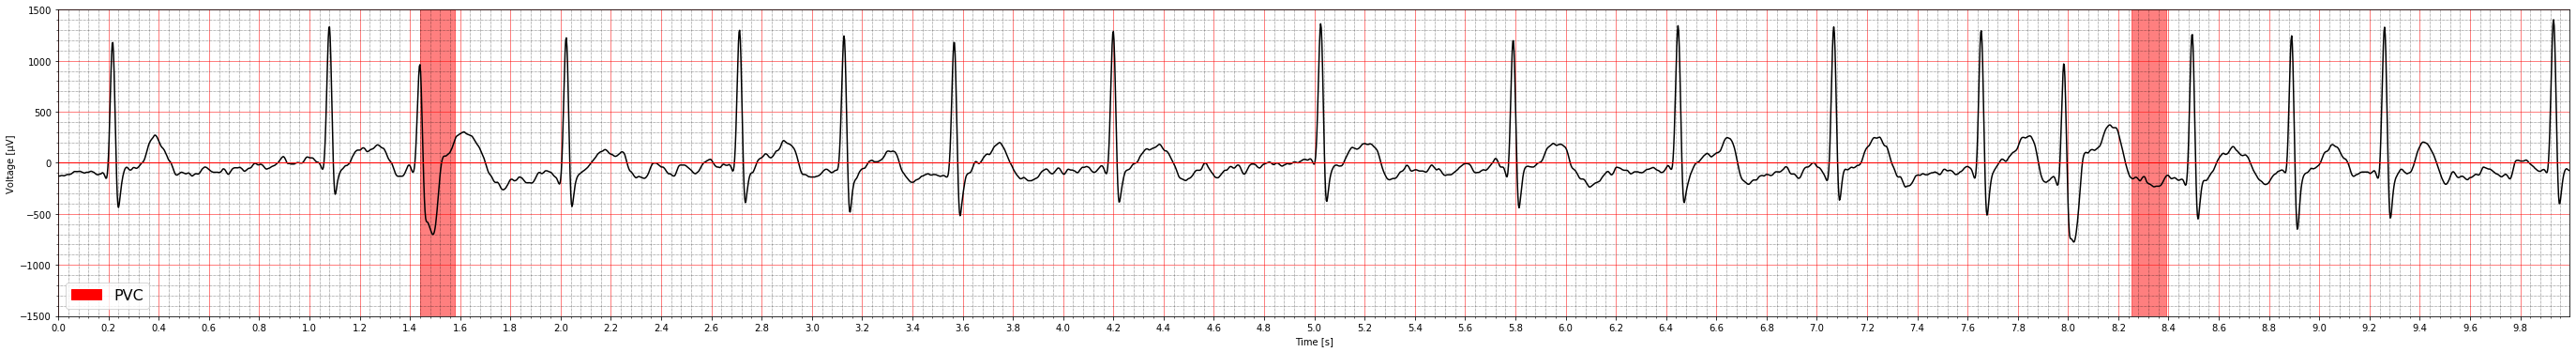
\includegraphics[width=\textwidth,keepaspectratio]{images/CPSC2020_A02_AF1.png}
\end{figure}
\end{block}

\uncover<6->{\bfseries 心律异常种类可高达上百种,且有可解释性的需求}

\end{frame}

%------------------------------------------------
% Page 15

\begin{frame}
\frametitle{深度学习应用于生理信号处理}

\begin{columns}

\begin{column}{0.72\textwidth}
\begin{block}{Motivation}<1->

\uncover<2->{{\large Stanford ML Group}}
\vspace{1em}

\uncover<3->{\textit{``Cardiologist-level arrhythmia detection and classification in ambulatory electrocardiograms using a deep neural network''}}
\vspace{1em}

\uncover<4->{{\large Nature Medicine}, volume 25, pages 65–69 (2019)}

\end{block}

\vspace{2.5em}

\uncover<3->{\raggedleft 模型结构:modified resnet34 $\rightarrow$}

\end{column}

\begin{column}{0.27\textwidth}
\uncover<3->{
\begin{figure}
    \centering
    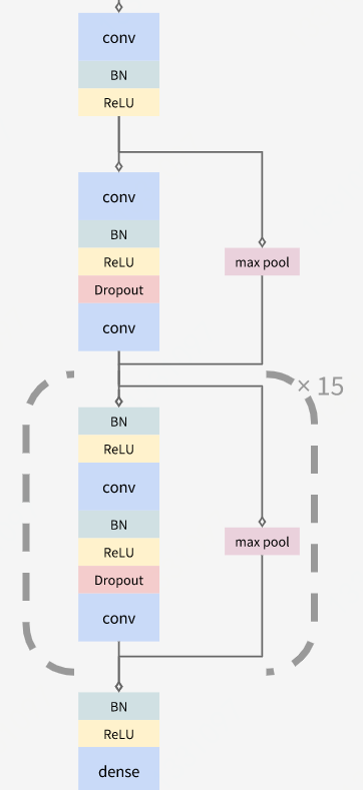
\includegraphics[width=\textwidth,keepaspectratio]{images/stanford_resnet34.png}
\end{figure}}
\end{column}

\end{columns}

\end{frame}

%------------------------------------------------
% Page 7

\begin{frame}
\frametitle{深度学习应用于生理信号处理}

\uncover<1->{
\begin{figure}
\centering
\begin{tikzpicture}[remember picture]
\node [rectangle] (resnet34) {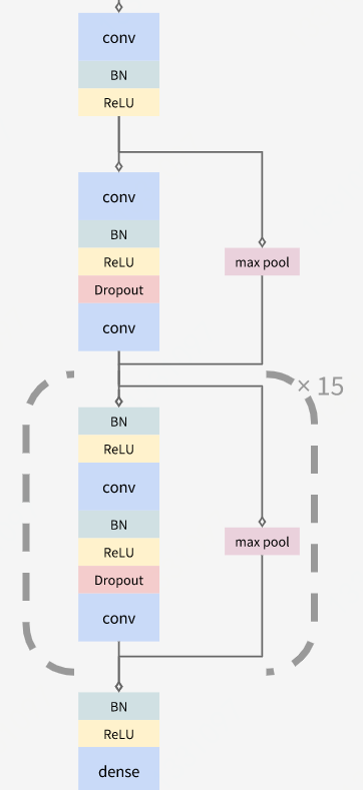
\includegraphics[width=0.27\textwidth,keepaspectratio]{images/stanford_resnet34.png}};
\node [rectangle, below left = 0.7cm and 1.7cm of resnet34.north] (cnn) {CNN};
\node [rectangle, below = 0.3cm of cnn.south] (resnet34_text) {resnet34};
\node [rectangle, below right = 0.7cm and 1.45cm of resnet34.north] (plus1) {
\includegraphics[width=0.05\textwidth,keepaspectratio]{images/gray_plus.png}};
\node [rectangle, below right = 0.7cm and 2.4cm of resnet34.north] (rnn) {RNN};
\node [rectangle, below = 0.7cm of rnn.south] (lstm) {{\footnotesize 双向LSTM}};
\node [rectangle, below = 0.5cm of lstm.south] (linear) {{\footnotesize Linear}};
\node [rectangle, below = 0.5cm of linear.south] (crf) {{\footnotesize \color{red} CRF}};
\node [rectangle, below right = 0.7cm and 3.55cm of resnet34.north] (plus2) {
\includegraphics[width=0.05\textwidth,keepaspectratio]{images/gray_plus.png}};
\node [rectangle, below right = 0.7cm and 4.4cm of resnet34.north] (pr) {``伪''PR间期后处理};
\node [rectangle, below = 1.1cm of pr.north] (pr_dist) {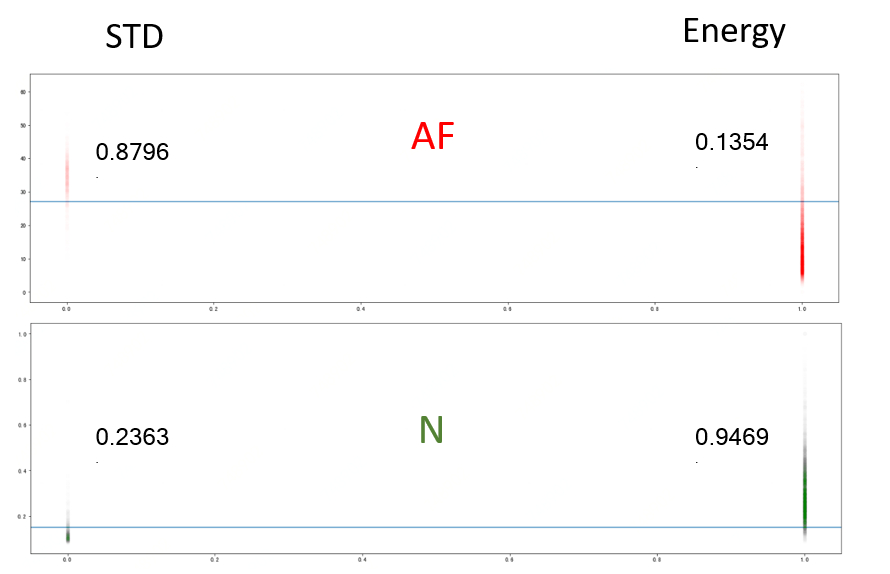
\includegraphics[width=0.37\textwidth,keepaspectratio]{images/pseudo_pr_dist_cinc2017.png}};

\path[->] ([yshift = -0.05cm]lstm.south) edge ([yshift = 0.05cm]linear.north);
\path[->] ([yshift = -0.05cm]linear.south) edge ([yshift = 0.05cm]crf.north);
\end{tikzpicture}
\end{figure}
}

\uncover<2->{
其他一些{\color{red}数据增强}{\color{zkblue} trick: random masking QRS complexes}
}

\end{frame}

%------------------------------------------------

\section{Blood Glucose Monitoring}

%------------------------------------------------
% Page 15

\begin{frame}


\end{frame}

%------------------------------------------------
% Page 15

\begin{frame}


\end{frame}

%------------------------------------------------

\section{NLP}

%------------------------------------------------
% Page 15

\begin{frame}


\end{frame}

%------------------------------------------------

\section{Miscellaneous}

%------------------------------------------------
% Page 15

\begin{frame}


\end{frame}

%------------------------------------------------
% Page 15

\begin{frame}
\frametitle{参考文献}



\end{frame}


%------------------------------------------------

% \begin{frame}

% \Huge{\centerline{\bfseries The End}}

% \vspace{0.5em}

% \Huge{\centerline{\phantom{a}\bfseries 谢谢!}}

% \end{frame}

%------------------------------------------------

\end{document}
